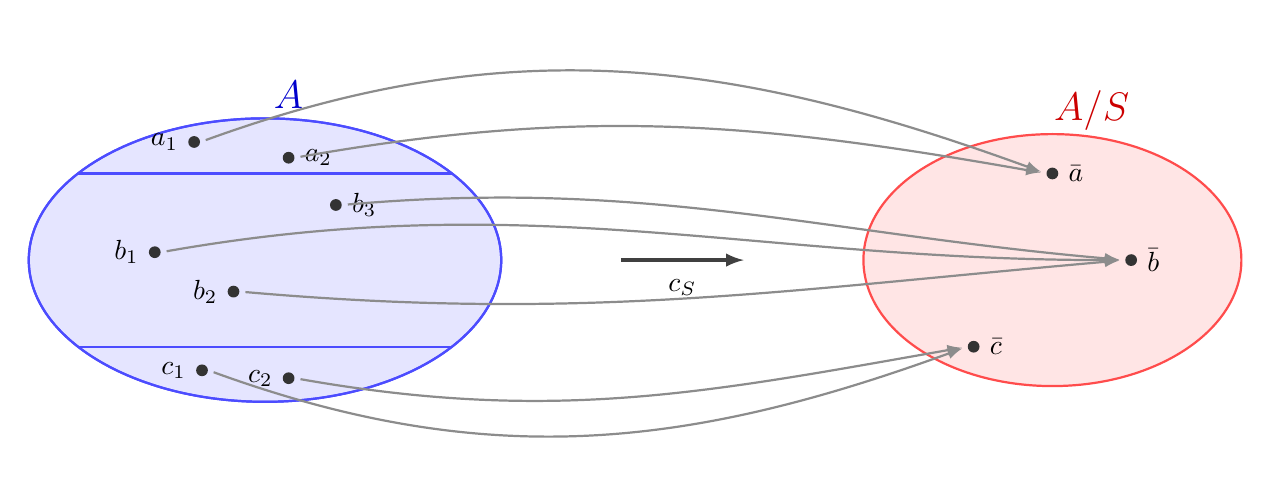
\begin{tikzpicture}[>=latex]

% --- Global TikZ Styles for Consistency ---
\tikzset{
    setA/.style={fill=blue!10, draw=blue!70, thick},
    setB/.style={fill=red!10, draw=red!70, thick},
    labelA/.style={text=blue!80!black, font=\Large\bfseries},
    labelB/.style={text=red!80!black, font=\Large\bfseries},
    partition/.style={draw=blue!70, thick},
    point/.style={circle, fill=black!80, inner sep=1.5pt},
    arrow/.style={
        ->,
        >=latex,
        thick,
        draw=black!45,
        shorten >=2pt,
        shorten <=2pt
    },
    mainarrow/.style={
        ->,
        >=latex,
        very thick,
        draw=black!75,
        shorten >=2pt,
        shorten <=2pt
    }
}

% Verzameling A
\path[setA] (0, 0) ellipse (3.0cm and 1.8cm);
\node[labelA] at (0.3, 2.1) {$A$};

% Partition Lines clipped inside A
\begin{scope}
    \clip (0, 0) ellipse (3.0cm and 1.8cm);
    \draw[partition] (-3.2, 1.1) -- (3.2, 1.1);
    \draw[partition] (-3.2, -1.1) -- (3.2, -1.1);
\end{scope}

% Redraw border of A so clipping does not visually affect the outline
\draw[blue!70, thick] (0, 0) ellipse (3.0cm and 1.8cm);

% Punten in A: top equivalence class
\node[point, label=left:$a_1$]  (at1) at (-0.9, 1.5) {};
\node[point, label=right:$a_2$] (at2) at (0.3, 1.3) {};
%\node[point, label=right:$a_3$] (at3) at (1.1, 1.5) {};

% Punten in A: middle equivalence class
\node[point, label=left:$b_1$]  (am1) at (-1.4, 0.1) {};
\node[point, label=left:$b_2$]  (am2) at (-0.4, -0.4) {};
\node[point, label=right:$b_3$] (am3) at (0.9, 0.7) {};
%\node[point, label=right:$b_4$] (am4) at (1.5, -0.1) {};

% Punten in A: bottom equivalence class
\node[point, label=left:$c_1$]  (ab1) at (-0.8, -1.4) {};
\node[point, label=left:$c_2$]  (ab2) at (0.3, -1.5) {};
%\node[point, label=right:$c_3$] (ab3) at (1.2, -1.4) {};

% Verzameling A/S
\path[setB] (10.0, 0) ellipse (2.4cm and 1.6cm);
\node[labelB] at (10.5, 1.9) {$A/S$};

% Punten in A/S
\node[point, label=right:$\bar{a}$] (bx) at (10.0, 1.1) {};
\node[point, label=right:$\bar{b}$] (by) at (11.0, 0.0) {};
\node[point, label=right:$\bar{c}$] (bz) at (9.0, -1.1) {};

% Canonical Quotient Mapping Arrow, centered between the two ellipses
% Right edge of A is x = 3.0, left edge of A/S is x = 7.6, midpoint is x = 5.3
\draw[mainarrow] (4.45, 0) -- (6.15, 0)
    node[midway, below=3pt] {$c_S$};

% Curved arrows from A to A/S: top class to X
\draw[arrow] (at1.east) to[out=20, in=160] (bx.west);
\draw[arrow] (at2.east) to[out=10, in=170] (bx.west);
%\draw[arrow] (at3.east) to[out=0,  in=180] (bx.west);

% Curved arrows from A to A/S: middle class to Y
\draw[arrow] (am1.east) to[out=10,  in=180] (by.west);
\draw[arrow] (am2.east) to[out=-5,  in=185] (by.west);
\draw[arrow] (am3.east) to[out=5,   in=175] (by.west);
%\draw[arrow] (am4.east) to[out=-10, in=190] (by.west);

% Curved arrows from A to A/S: bottom class to Z
\draw[arrow] (ab1.east) to[out=-20, in=200] (bz.west);
\draw[arrow] (ab2.east) to[out=-10, in=190] (bz.west);
%\draw[arrow] (ab3.east) to[out=0,   in=180] (bz.west);

\end{tikzpicture}